% Level ceiling (grade 6): density handled as "mass of one cubic
% centimetre" via proportionality tables and division; the literal
% formula rho = m/V waits for grade 7 (literal expressions, math g7).
\chapter{密度：为什么物体会漂浮}\label{ch:g6:density-floating}

在你刚入学的第一年，一枚小硬币沉了下去，而一根大木头却浮了起来，
我们曾承诺，“为什么”正是本课程的宝藏。
你已经赢得了它。钥匙是在前两章里锻造成的，
物质看\omterm{def:g3:measuring-mass:mass}{质量}，房间看\omterm{def:g6:mass-and-volume:volume}{体积}——今天这两者
在这把锁上合力转动。

\section{一立方厘米的质量}

\begin{example}[终于可以公平比较]\label{ex:g6:density-floating:fair}
把整根木头和整枚硬币放在一起比，从来都不公平：
大小不同，形状也不同。公平的比赛应当取\emph{相同
\omterm{def:g6:mass-and-volume:volume}{体积}}：每位参赛者各取一\omterm{def:g6:mass-and-volume:volume}{立方厘米}。
一 \unit{cm^3} 水的\omterm{def:g3:measuring-mass:mass}{质量}为 \qty{1}{g}；一 \unit{cm^3}
的橡木约 \qty{0.6}{g}；石头约 \qty{2.5}{g}；
铁为 \qty{7.9}{g}。空间相同，物质却千差万别——这正是
浮沉游戏一直在等待的那个数字。
\end{example}

\begin{definition}[密度]\label{def:g6:density-floating:density}
某种物质的\emph{密度}\index{密度}，是指
该物质一\omterm{def:g6:mass-and-volume:volume}{立方厘米}的\omterm{def:g3:measuring-mass:mass}{质量}，\omterm{def:g6:measurement-in-science:measuring}{单位}为克。水的密度是
\qty{1}{g} 每 \unit{cm^3}；橡木约 $0.6$；铁为 $7.9$。求
密度不需要新仪器：只需测出样品的
\omterm{def:g3:measuring-mass:mass}{质量}和\omterm{def:g6:mass-and-volume:volume}{体积}，然后相除——把克数平均分给各\omterm{def:g6:mass-and-volume:volume}{立方厘米}，
答案便是每\omterm{def:g6:mass-and-volume:volume}{立方厘米}所得的
份额。
\end{definition}

\begin{omfigure}
\begin{tikzpicture}[scale=0.85]
  \foreach \x/\name/\m/\c in {0.9/软木/0.2/omMeth,
      3.0/橡木/0.6/omMeth, 5.1/水/1.0/omDef,
      7.2/石头/2.5/omExo, 9.3/铁/7.9/omThm} {
    \draw[thick, fill=\c, fill opacity=0.4]
      (\x,0.6) rectangle ++(1.0,1.0);
    \node[above, font=\footnotesize] at (\x+0.5,1.65) {\name};
    \node[below, font=\footnotesize] at (\x+0.5,0.5)
      {$\m$ g};
  }
  \node[below, font=\small] at (5.6,-0.15)
    {五块相同的一立方厘米方块——五种质量};
\end{tikzpicture}

{\small 公平的比赛：每人空间相同，每种
物质都显出自己的“特征\omterm{def:g3:measuring-mass:mass}{质量}”。}
\end{omfigure}

\begin{proposition}[密度是特征]\label{prop:g6:density-floating:signature}
纯净物质的\omterm{def:g6:density-floating:density}{密度}，对其任一部分都相同，
无论大小：一小块橡木和一整根横梁，都是
每\omterm{def:g6:mass-and-volume:volume}{立方厘米}约 \qty{0.6}{g}。因此，\omterm{def:g6:density-floating:density}{密度}可以识别物质，
与\omterm{def:g4:changes-of-state:melting-point}{熔点}一样：测出一个不明物体的
\omterm{def:g3:measuring-mass:mass}{质量}和\omterm{def:g6:mass-and-volume:volume}{体积}，相除后与表格对照——
物质往往当场就能“招供”。
\end{proposition}

\begin{method}[测量密度]\label{met:g6:density-floating:measure}
对于一块卵石——或一顶王冠：
\begin{enumerate}
  \item 用\omterm{def:g3:levers-and-scales:scale}{天平}测出它的\omterm{def:g3:measuring-mass:mass}{质量}，比如 \qty{75}{g}；
  \item 用水面上升法测出它的\omterm{def:g6:mass-and-volume:volume}{体积}，比如
        \qty{30}{cm^3};
  \item 把克数除以\omterm{def:g6:mass-and-volume:volume}{立方厘米}数：$75 \div 30 =
        2.5$——每\omterm{def:g6:mass-and-volume:volume}{立方厘米}含 \qty{2.5}{g}；
  \item 查表：\omterm{def:g6:density-floating:density}{密度}为 $2.5$——这块卵石是
        普通的石头。
\end{enumerate}
\end{method}

\section{浮沉规律}

\begin{proposition}[物体为什么会漂浮]\label{prop:g6:density-floating:rule}
物体在水中\omterm{def:g1:floating-and-sinking:words}{漂浮}，若其\omterm{def:g6:density-floating:density}{密度}\emph{小于}
水的\omterm{def:g6:density-floating:density}{密度}——即每\omterm{def:g6:mass-and-volume:volume}{立方厘米}不足 \qty{1}{g}——，
若\omterm{def:g6:density-floating:density}{密度}更大则\omterm{def:g1:floating-and-sinking:words}{下沉}。可以说，水在把闯入者与自身
逐\omterm{def:g6:mass-and-volume:volume}{体积}地比较：每\omterm{def:g6:measurement-in-science:measuring}{单位}\omterm{def:g6:mass-and-volume:volume}{体积}比水轻的浮在上面；
每\omterm{def:g6:measurement-in-science:measuring}{单位}\omterm{def:g6:mass-and-volume:volume}{体积}比水重的则沉下去。同样的规律适用于
任何\omterm{def:g3:solids-liquids-gases:liquid}{液体}，各自以其\omterm{def:g6:density-floating:density}{密度}作为裁判。
\end{proposition}

\begin{omfigure}
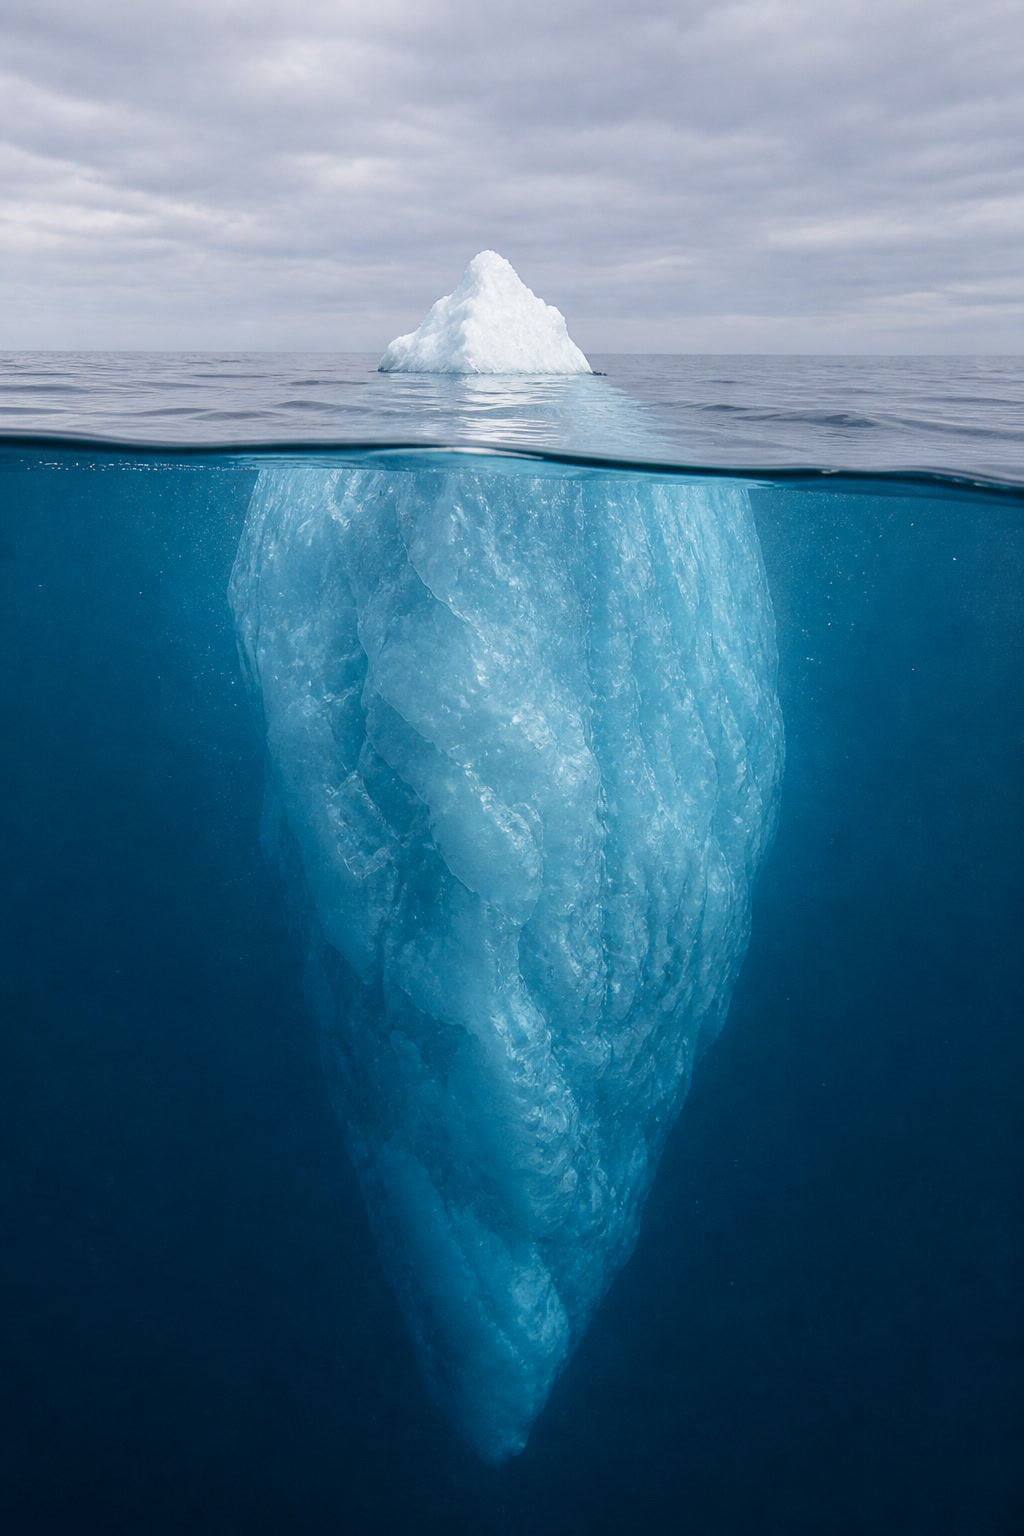
\includegraphics[width=0.4\linewidth]{images/book1/ai/g6-density-iceberg.jpg}

{\small 冰的\omterm{def:g6:density-floating:density}{密度}只略小于水——因此冰山\omterm{def:g1:floating-and-sinking:words}{漂浮}时，大部分\omterm{def:g6:mass-and-volume:volume}{体积}隐藏在水面以下。}
\end{omfigure}

\begin{example}[六年谜题，终于解开]\label{ex:g6:density-floating:settled}
木头（$0.6$）：无论多大都会\omterm{def:g1:floating-and-sinking:words}{漂浮}——它的每\omterm{def:g6:mass-and-volume:volume}{立方厘米}
都比水轻。硬币（青铜，约 $9$）：无论多小都会
\omterm{def:g1:floating-and-sinking:words}{下沉}。塑料鸭、软木塞、铅笔：\omterm{def:g6:density-floating:density}{密度}都在 $1$ 以下，
统统是\omterm{def:g1:floating-and-sinking:words}{漂浮}者。冰，\omterm{def:g6:density-floating:density}{密度}为 $0.9$——水自己膨胀后的\omterm{def:g3:solids-liquids-gases:solid}{固体}——
在自身的\omterm{def:g3:solids-liquids-gases:liquid}{液体}上勉强浮着，只差一丝，所以池塘常盖着
冰盖，冰山才能漂航。那么橡皮泥小船呢？做成
碗形，\emph{船加\omterm{def:g2:air-around-us:air}{空气}}这一整体\omterm{def:g6:measurement-in-science:measuring}{单位}\omterm{def:g6:mass-and-volume:volume}{体积}内含\omterm{def:g2:air-around-us:air}{空气}很多：
整体的\omterm{def:g6:density-floating:density}{密度}降到 $1$ 以下，而在码头上，
同样的诀窍让一艘艘万吨钢船下水。
\end{example}

\begin{omfigure}
\begin{tikzpicture}[scale=0.85]
  \draw[thick] (0.8,0) -- (0.8,3.4) (4.0,0) -- (4.0,3.4)
    (0.8,0) -- (4.0,0);
  \fill[omMeth, opacity=0.35] (0.8,2.2) rectangle (4.0,3.0);
  \node[font=\footnotesize] at (2.4,2.6) {油：$0.9$};
  \fill[omDef, opacity=0.3] (0.8,1.1) rectangle (4.0,2.2);
  \node[font=\footnotesize] at (2.4,1.65) {水：$1.0$};
  \fill[omThm, opacity=0.3] (0.8,0.05) rectangle (4.0,1.1);
  \node[font=\footnotesize] at (2.4,0.55) {蜂蜜：$1.4$};
  \node[below, font=\small] at (2.4,-0.3)
    {液体分层：底部密度最大};
  \draw[thick] (7.2,0) -- (7.2,3.4) (11.0,0) -- (11.0,3.4)
    (7.2,0) -- (11.0,0);
  \fill[omDef, opacity=0.3] (7.2,0.05) rectangle (11.0,2.6);
  \draw[thick, fill=white]
    (8.3,2.35) -- (9.9,2.35) -- (9.6,2.95) -- (8.6,2.95) -- cycle;
  \draw[thick, fill=white, fill opacity=0.7]
    (8.0,2.35) -- (10.2,2.35) -- (9.5,1.0) -- (8.7,1.0) -- cycle;
  \node[font=\footnotesize] at (9.1,1.85) {冰：$0.9$};
  \node[below, font=\small] at (9.1,-0.3)
    {冰山：十分之九在水面以下};
\end{tikzpicture}

{\small \omterm{def:g6:density-floating:density}{密度}的“笔迹”：\omterm{def:g3:solids-liquids-gases:liquid}{液体}按\omterm{def:g6:density-floating:density}{密度}由大到小自下而上分层，
冰（$0.9$）浮在水面上时，仅十分之一露出水面。}
\end{omfigure}

\begin{example}[液体塔]\label{ex:g6:density-floating:tower}
先把蜂蜜，再把染了墨的水，最后把油，沿着高玻璃杯的内壁轻轻倒入，
形成三层：蜂蜜（$1.4$）在底部，油
（$0.9$）在顶部，它们各守层次，互不相混。放入几位“客人”：一颗
葡萄（$1.05$）先穿过油\omterm{def:g1:floating-and-sinking:words}{下沉}，再穿过水\omterm{def:g1:floating-and-sinking:words}{下沉}，
最后停在蜂蜜层上——它比油和水都密，却比蜂蜜轻。
这座“\omterm{def:g3:solids-liquids-gases:liquid}{液体}塔”把浮沉规律演成了一出戏。
\end{example}

\begin{remark}[读懂冰山]\label{rem:g6:density-floating:iceberg}
冰的 $0.9$ 与水的 $1.0$ 相比，不仅使冰山浮起，
它还决定了水线的位置。冰山十分之九的\omterm{def:g6:mass-and-volume:volume}{体积}位于
\emph{水面以下}——正是那块隐藏的\omterm{def:g3:measuring-mass:mass}{质量}，
曾使不少自负的船只沉没。水下部分的比例究竟\emph{为何}恰好等于
\omterm{def:g6:density-floating:density}{密度}之比，这是一条优美的定律，由阿基米德
本人发现，其严格证明将在高中分册中给出；
\omterm{def:g6:density-floating:density}{密度}表已经暗示了答案。
\end{remark}

\section{王冠，终于揭晓}

\begin{example}[阿基米德破案]\label{ex:g6:density-floating:crown}
现在来讲完两章前开始的故事。王冠的\omterm{def:g3:measuring-mass:mass}{质量}：
容易，\omterm{def:g3:levers-and-scales:scale}{天平}即可测得。它的\omterm{def:g6:mass-and-volume:volume}{体积}：对于形状不规则的
工艺品而言难以直接\omterm{def:g6:measurement-in-science:measuring}{测量}——直到“澡盆”的启示给出了排水法。
\omterm{def:g3:measuring-mass:mass}{质量}除以\omterm{def:g6:mass-and-volume:volume}{体积}：王冠的\emph{\omterm{def:g6:density-floating:density}{密度}}——
而\omterm{def:g6:density-floating:density}{密度}就是一种“指纹”。纯金的为 $19.3$；白银的为
$10.5$；某种秘密配比的合金则介于两者之间。传说
金匠的王冠“招认”出的\omterm{def:g6:density-floating:density}{密度}远低于纯金，
骗局就此被揭穿，王冠却毫发无损。
周末问题给出了他的数据。
\end{example}

\section{练习}

\begin{exercise}[$\star$]\label{exo:g6:density-floating:1}
什么是物质的\omterm{def:g6:density-floating:density}{密度}？写出水的\omterm{def:g6:density-floating:density}{密度}，并叙述
浮沉规律。
\end{exercise}

\begin{exercise}[$\star$]\label{exo:g6:density-floating:2}
预测下列物体放入水中是上浮还是\omterm{def:g1:floating-and-sinking:words}{下沉}：橡木（$0.6$）；\ 石头（$2.5$）；\
软木（$0.2$）；\ 铁（$7.9$）；\ 冰（$0.9$）。
\end{exercise}

\begin{exercise}[$\star$]\label{exo:g6:density-floating:3}
一块物体的\omterm{def:g3:measuring-mass:mass}{质量}为 \qty{120}{g}，\omterm{def:g6:mass-and-volume:volume}{体积}为 \qty{80}{cm^3}。求它的
\omterm{def:g6:density-floating:density}{密度}，它放入水中会上浮还是\omterm{def:g1:floating-and-sinking:words}{下沉}？
\end{exercise}

\begin{exercise}[$\star$]\label{exo:g6:density-floating:4}
一块神秘的物块：\omterm{def:g3:measuring-mass:mass}{质量}为 \qty{158}{g}，放入量筒后液面上升
\qty{20}{cm^3}。求它的\omterm{def:g6:density-floating:density}{密度}，并根据本章的数据，
推断它可能是哪种物质？
\end{exercise}

\begin{exercise}[$\star$]\label{exo:g6:density-floating:5}
为什么一小块橡木的\omterm{def:g6:density-floating:density}{密度}与整根橡木梁
的\omterm{def:g6:density-floating:density}{密度}相同？这一性质有什么用处？
\end{exercise}

\begin{exercise}[$\star$]\label{exo:g6:density-floating:6}
在\omterm{def:g3:solids-liquids-gases:liquid}{液体}塔中，为什么蜂蜜在最下面，油在
上面？\omterm{def:g6:density-floating:density}{密度}为 $1.05$ 的葡萄会停在哪里？
\end{exercise}

\begin{exercise}[$\star$]\label{exo:g6:density-floating:7}
冰能浮在水面上——对于\omterm{def:g3:solids-liquids-gases:solid}{固体}来说，这为什么是反常的？
哪一条关于水\omterm{def:g6:water-states:changes}{凝固}的古老命题可以解释冰的 $0.9$？
\end{exercise}

\begin{exercise}[$\star$]\label{exo:g6:density-floating:8}
七年级时学过的“大木头”和“小硬币”：给出
最终、完整的答案，并利用本章的数据。
\end{exercise}

\begin{exercise}[$\star\star$]\label{exo:g6:density-floating:9}
某种\omterm{def:g3:solids-liquids-gases:liquid}{液体}一升的\omterm{def:g3:measuring-mass:mass}{质量}为 \qty{800}{g}。以克每\omterm{def:g6:mass-and-volume:volume}{立方厘米}为\omterm{def:g6:measurement-in-science:measuring}{单位}，它的
\omterm{def:g6:density-floating:density}{密度}是多少？一块冰块
（$0.9$）放入其中会上浮还是\omterm{def:g1:floating-and-sinking:words}{下沉}？
\end{exercise}

\begin{exercise}[$\star\star$]\label{exo:g6:density-floating:10}
钢的\omterm{def:g6:density-floating:density}{密度}为 $7.9$，但钢船却能浮在水面上。请运用
借助
\cref{ex:g6:density-floating:settled}中的“包裹”思想——除了钢，船上的“包裹”还包括什么，
以及其整体\omterm{def:g6:density-floating:density}{密度}必须为多少？
破损的船何时不再满足这一规律？
\end{exercise}

\begin{exercise}[$\star\star$]\label{exo:g6:density-floating:11}
海水的\omterm{def:g6:density-floating:density}{密度}比淡水略大，约为 $1.03$。
解释为什么人在海水中\omterm{def:g1:floating-and-sinking:words}{漂浮}得明显更好，并预测
一艘船从咸海驶入淡水河时，
其水线会如何变化。
\end{exercise}

\begin{exercise}[$\star\star\star$]\label{exo:g6:density-floating:12}
一个空心金属球恰好有一半浸在水中\omterm{def:g1:floating-and-sinking:words}{漂浮}。
推算\emph{整个球形“包裹”}（金属
外壳加内部\omterm{def:g2:air-around-us:air}{空气}）的\omterm{def:g6:density-floating:density}{密度}。然后论证，若水缓慢渗入
球内，它会向哪个方向运动，并说明在什么时刻开始\omterm{def:g1:floating-and-sinking:words}{下沉}
——请同时运用规律与“包裹”的思想。
\end{exercise}

\section{周末问题：国王的王冠}

\begin{problem}[{周末问题——国王王冠一案，
用你的仪器重新审视；金匠的审判，
借除法破解}]\label{pb:g6:density-floating:1}
用现代数据重新审视古代最著名的欺诈案。
特征数据：金 $19.3$，银 $10.5$（
克每\omterm{def:g6:mass-and-volume:volume}{立方厘米}）。

\medskip\noindent\textbf{第一部分——证据。}
国王交给金匠 \qty{1930}{g} 纯金。
做成的王冠放在\omterm{def:g3:levers-and-scales:scale}{天平}上，\omterm{def:g3:measuring-mass:mass}{质量}恰好为 \qty{1930}{g}。
\begin{enumerate}
  \item \omterm{def:g3:measuring-mass:mass}{质量}完全吻合。为什么仅凭这一点
        无法说明任何欺诈问题？（金匠能做什么，
        仍能使\omterm{def:g3:measuring-mass:mass}{质量}吻合？）
  \item \qty{1930}{g} 的\emph{纯金}应占多大\omterm{def:g6:mass-and-volume:volume}{体积}？
        （把克数分组：每组
        \qty{19.3}{g}，可占几\omterm{def:g6:mass-and-volume:volume}{立方厘米}？）
  \item 阿基米德将王冠放入盛满水的容器中，
        收集溢出的水，其\omterm{def:g6:mass-and-volume:volume}{体积}为 \qty{130}{cm^3}。
        王冠的真实\omterm{def:g6:mass-and-volume:volume}{体积}是多少？
  \item 比较两个\omterm{def:g6:mass-and-volume:volume}{体积}。这一比较已经
        说明了什么？
\end{enumerate}

\medskip\noindent\textbf{第二部分——特征数据。}
\begin{enumerate}[resume]
  \item 由王冠的\omterm{def:g3:measuring-mass:mass}{质量}和测得的\omterm{def:g6:mass-and-volume:volume}{体积}，
        计算王冠的\omterm{def:g6:density-floating:density}{密度}（保留一位小数即可）。
  \item 将三个特征数据并列比较：金、王冠、
        银。王冠的\omterm{def:g6:density-floating:density}{密度}落在何处？
  \item 用一句话向国王解释，王冠为何
        不可能是纯金。
  \item 金匠抗议：“也许是\omterm{def:g3:levers-and-scales:scale}{天平}出错了！”
        姑且给他宽限，允许\omterm{def:g3:levers-and-scales:scale}{天平}向任一方向有 \qty{30}{g} 的误差。
        在 \qty{1900}{g} 与 \qty{1960}{g} 之间，
        能否使\omterm{def:g6:mass-and-volume:volume}{体积}为 \qty{130}{cm^3} 的纯金王冠得以“开脱”？
        （请检验\omterm{def:g6:density-floating:density}{密度}范围。）
\end{enumerate}

\medskip\noindent\textbf{第三部分——究竟偷了多少？}
假设金匠私吞了一部分黄金，并以银按
同样的克数予以替换。
\begin{enumerate}[resume]
  \item 以银替换金，按相同克数替换，
        \omterm{def:g3:measuring-mass:mass}{质量}仍然正确，\omterm{def:g6:mass-and-volume:volume}{体积}却为何会\emph{膨胀}？
  \item 检验一个猜想：一顶王冠由 \qty{965}{g} 金 $+$
        \qty{965}{g} 银组成。金的部分\omterm{def:g6:mass-and-volume:volume}{体积}是多少？
        银的部分\omterm{def:g6:mass-and-volume:volume}{体积}是多少？（保留一位小数。）
  \item 求出猜想中王冠的总\omterm{def:g6:mass-and-volume:volume}{体积}，并以
        实测的 \qty{130}{cm^3} 检验此猜想：银是多了，还是
        少了？
  \item 法庭需要一句判决：陈述已被毫无疑问证明的
        结论（是否为纯金），所用的方法是什么，
        以及王冠为何无需受损 ——
        这正是阿基米德真正的胜利。
\end{enumerate}
\end{problem}
